% This is samplepaper.tex, a sample chapter demonstrating the
% LLNCS macro package for Springer Computer Science proceedings;
% Version 2.20 of 2017/10/04
%
\documentclass[runningheads]{llncs}
%
\usepackage[export]{adjustbox}
\usepackage{graphicx}
\usepackage{biblatex}
\addbibresource{ref.bib}
% Used for displaying a sample figure. If possible, figure files should
% be included in EPS format.
%
% If you use the hyperref package, please uncomment the following line
% to display URLs in blue roman font according to Springer's eBook style:
% \renewcommand\UrlFont{\color{blue}\rmfamily}

\begin{document}
%
\title{The Influence of LIWC Features in the Detection of Fake News}
%
%\titlerunning{Abbreviated paper title}
% If the paper title is too long for the running head, you can set
% an abbreviated paper title here
%
\author{Nicolas Gonzalez Albo Mendez
%
\authorrunning{F. Author et al.}
% First names are abbreviated in the running head.
% If there are more than two authors, 'et al.' is used.
%
\institute{Monterrey Institute of Technology and Higher Education, Atlixcayotl 5718, Reserva Territorial Atlixcayotl, 72453, Puebla, Mexico}
\email{A01730763@itesm.mx}}

%
\maketitle              % typeset the header of the contribution
%
\begin{abstract}
In a society were we use social media vastly in our life, many overwhelming quantities of information are being consumed by us. Most of the news in recent times are viral because of social networks. Therefore, they need to have the same disposable characteristics as other data in social networks. This has exposed us to be vulnerable to the vast amount of news out because of its volatile nature, we rarely fact check them or even stop to read in detain. Fake news detection algorithms offer a potential solution to this problem. In this work, given a training and testing database with news in text we explored the performance of classifiers LMT, DecisionTree, Logistic Regression and Multilayer Perceptron fed with a relatively big amount of 161 features exctracted from MeaningCloud, ParallelDots and Receptivity APIs. These features were later reduced into a smaller but more score-impacting pool using Cfs Subset Evaluator. Results were evaluated using the score of a Kaggle competition named "Detecting fake news". At the end, after comparing the classifiers mentioned earlier, the best classifier was LMT which performed better when evaluating the attributes and reducing them to 17, obtaining a score of 0.97500 in the competition, finishing in first place. LMT outperformed Random Forest ant the end by just 0.01 points in score, which indicates the robustness of this other classifier.

\keywords{First keyword  \and Second keyword \and Another keyword.}
\end{abstract}
%
%
%
\section{Introduction}
In the past, the problem humanity was facing, was the lack of information. There were not enough ways for people to get reliable and accurate information. Nowadays, we are facing the opposite situation, we live in an era of over-information, news about every topic of every domain can be found in the internet, from politics and finance to celebrities' gossip. The problem of this massive amount of news is that not all news are legitimate, therefore people may believe that certain information is real when it is not.

The problem is not only the consumption of fake news, but also the propagation of them. In fact, a report from the Jumpshot Tech Blog found that 50\% of non-legitimate news sites and 20\% of reputable websites total traffic came from Facebook referrals, also 62\% of American adults gets news on social media (Jeffrey and Elisa, 2016), being said that, it can be inferred that most of the fake news in the United States are shared by adults through social media. 

Until know, the majority of computational approaches for fake news detection have relied on satirical news such as "The Onion" or and fact-checking websites such as "poliFact" and "Snopes". The problem of using such websites as sources for fake news is that many confounding factors are brought into the analysis like humor or absurdity.

This paper is written due to the necessity of creating an effective fake news detector. It incorporates the use of sentiment, emotions and linguistic features that achieve accuracies up to 97.5\%. These features were extracted two datasets: training and training. Different supervised learning algorithms were used and compared for classifying fake news.

\section{Related Works}
Big efforts from different researchers have been made around the globe, these are some works that have been made in the field of machine learning for the detection of fake news.

\subsection{Automatic Detection of Fake News}
The authors of this paper realized the construction of two novel datasets covering seven different domains of interest. One of the datasets was collected through a combination of manual and crowdsourced annotation efforts and includes news from six different domains (sports, business, entertainment, politics, technology and education), whereas the second dataset was collected directly from the web and was limited to a single domain (Celebrity news). 

Different analyses where conducted to identify linguistic features that are predominant in fake news, resulting in the creation of fake news detectors that achieve accuracies up to 78\%. These analyses where conducted with different combinations of feature sets and a linear SVM classifier was used along with a five-fold cross-validation. The entirety of the machine learning classification process was made with R. 

Important results from this papers are that humans are better at detecting fake information in celebrity news, but the system they built outperformed humans in the detection of fake news in more serious domains like politics or businesses.
\subsection{DETECTIVE Algorithm}
Is an algorithm proposed in 2018 for the detection of fake news. As described by its authors:
\paragraph{"It works by actively trading off between exploration and exploitation by the use of posterior sampling (Thompson sampling). In each invocation, the algorithm samples the user's parameters from the current users' posterior distributions and invokes TopX with these parameters"}. \\

This approach can be imagined like sampling users' parameters that are related to the probability they are optimal". 

\begin{figure}[hbt!]
\centering
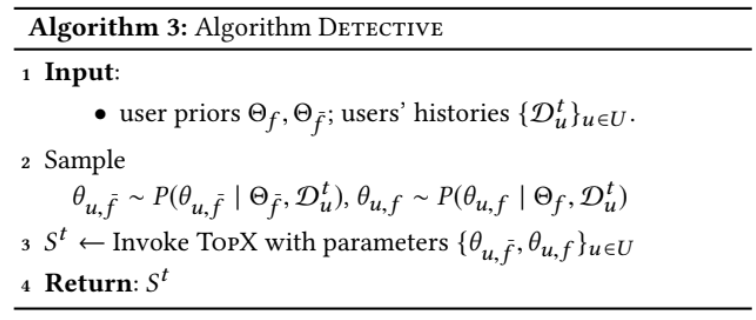
\includegraphics[width=10cm, height=5cm]{DETECTIVE.png}
\caption{Mathematical model of DETECTIVE algorithm}
\end{figure}


\section{Our proposal}
In this work, a different approach for developing a fake news detector was implemented. It originally used 161 features, excluding the ID and the class, related to sentiments, emotions, intent and linguistics. These features were extracted from different APIs (MeaningCloud, ParallelDots and Receptivity) using Python.

After a preprocessor was applied, the number of features drastically dropped to only 17. Different classifiers where used like LMT, DecisionTree, Logistic Regression and Multilayer Perceptron.

\section{Experimental setup}
Two different scripts were developed for extracting the data from the different APIs. The first script extracted data related to sentiments, emotions and intent using MeaningCloud for the first group of features and ParallelDots for the other two. The second script extracted data related to linguistics using the Receptivity API, this API classified the features of the dataset news based on the LIWC (Linguistic Inquiry and Word Count)and SALLEE (Syntax-Aware LexicaL Emotion Engine; pronounced “Sally”) lexical engines. 

After that, by using WEKA, different classifiers were used in order to achieve a higher score. Also a CfsSubsetEval preproccesor was used in order to improve the score in Kaggle. 

\section{Experimental results and discussion}
By trying different classifiers with only 15 features related to sentiments, emotions and intent, the classifier that obtained the best score was a logistic regression with a score of 0.68055

\begin{figure}[hbt!]
\centering
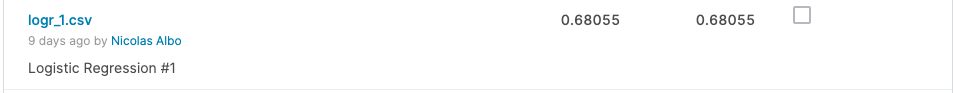
\includegraphics[width=12cm, height=1.5cm]{logreg1.png}
\caption{Score obtained by a Logistic Regression classifier in Kaggle using 15 features.}
\end{figure}

Then, at seeing no results with the current number of features, it was decided to extract new features. So, 146 features related to linguistics were extracted, this decision was influenced by the paper \emph{Automatic Detection of Fake News}, were the authors used several linguistic features for the creation of fake news detectors. 

By using again a Logistic Regression classifier with both the old and new features, a new highscore of 0.89166 was obtained in Kaggle.

\begin{figure}[hbt!]
\centering

\includegraphics[width=12cm, height=1.5cm]{logreg2.png}
\caption{Score obtained by a Logistic Regression classifier in Kaggle with both old and new features}
\end{figure}

Not satisfied by the previous score obtained in Kaggle, it was decided to try different classifiers, where a Random Forest of 165 features obtained a higher score with 0.96666.

\begin{figure}[hbt!]
\centering

\includegraphics[width=12cm, height=1.5cm]{RandomForest1.png}
\caption{Score obtained by a Random Forest classifier in Kaggle with both old and new features}
\end{figure}

It was supposed that not all of the features were contributing to obtain a higher score, so it was applied a preprocess to the current features in order to see which were relevant and which not. Then, it resulted that by using a CfsSubsetEval Attribute Evaluator, only 17 of the 165 features were relevant for the detection of fake news.

\begin{figure}[hbt!]
\centering
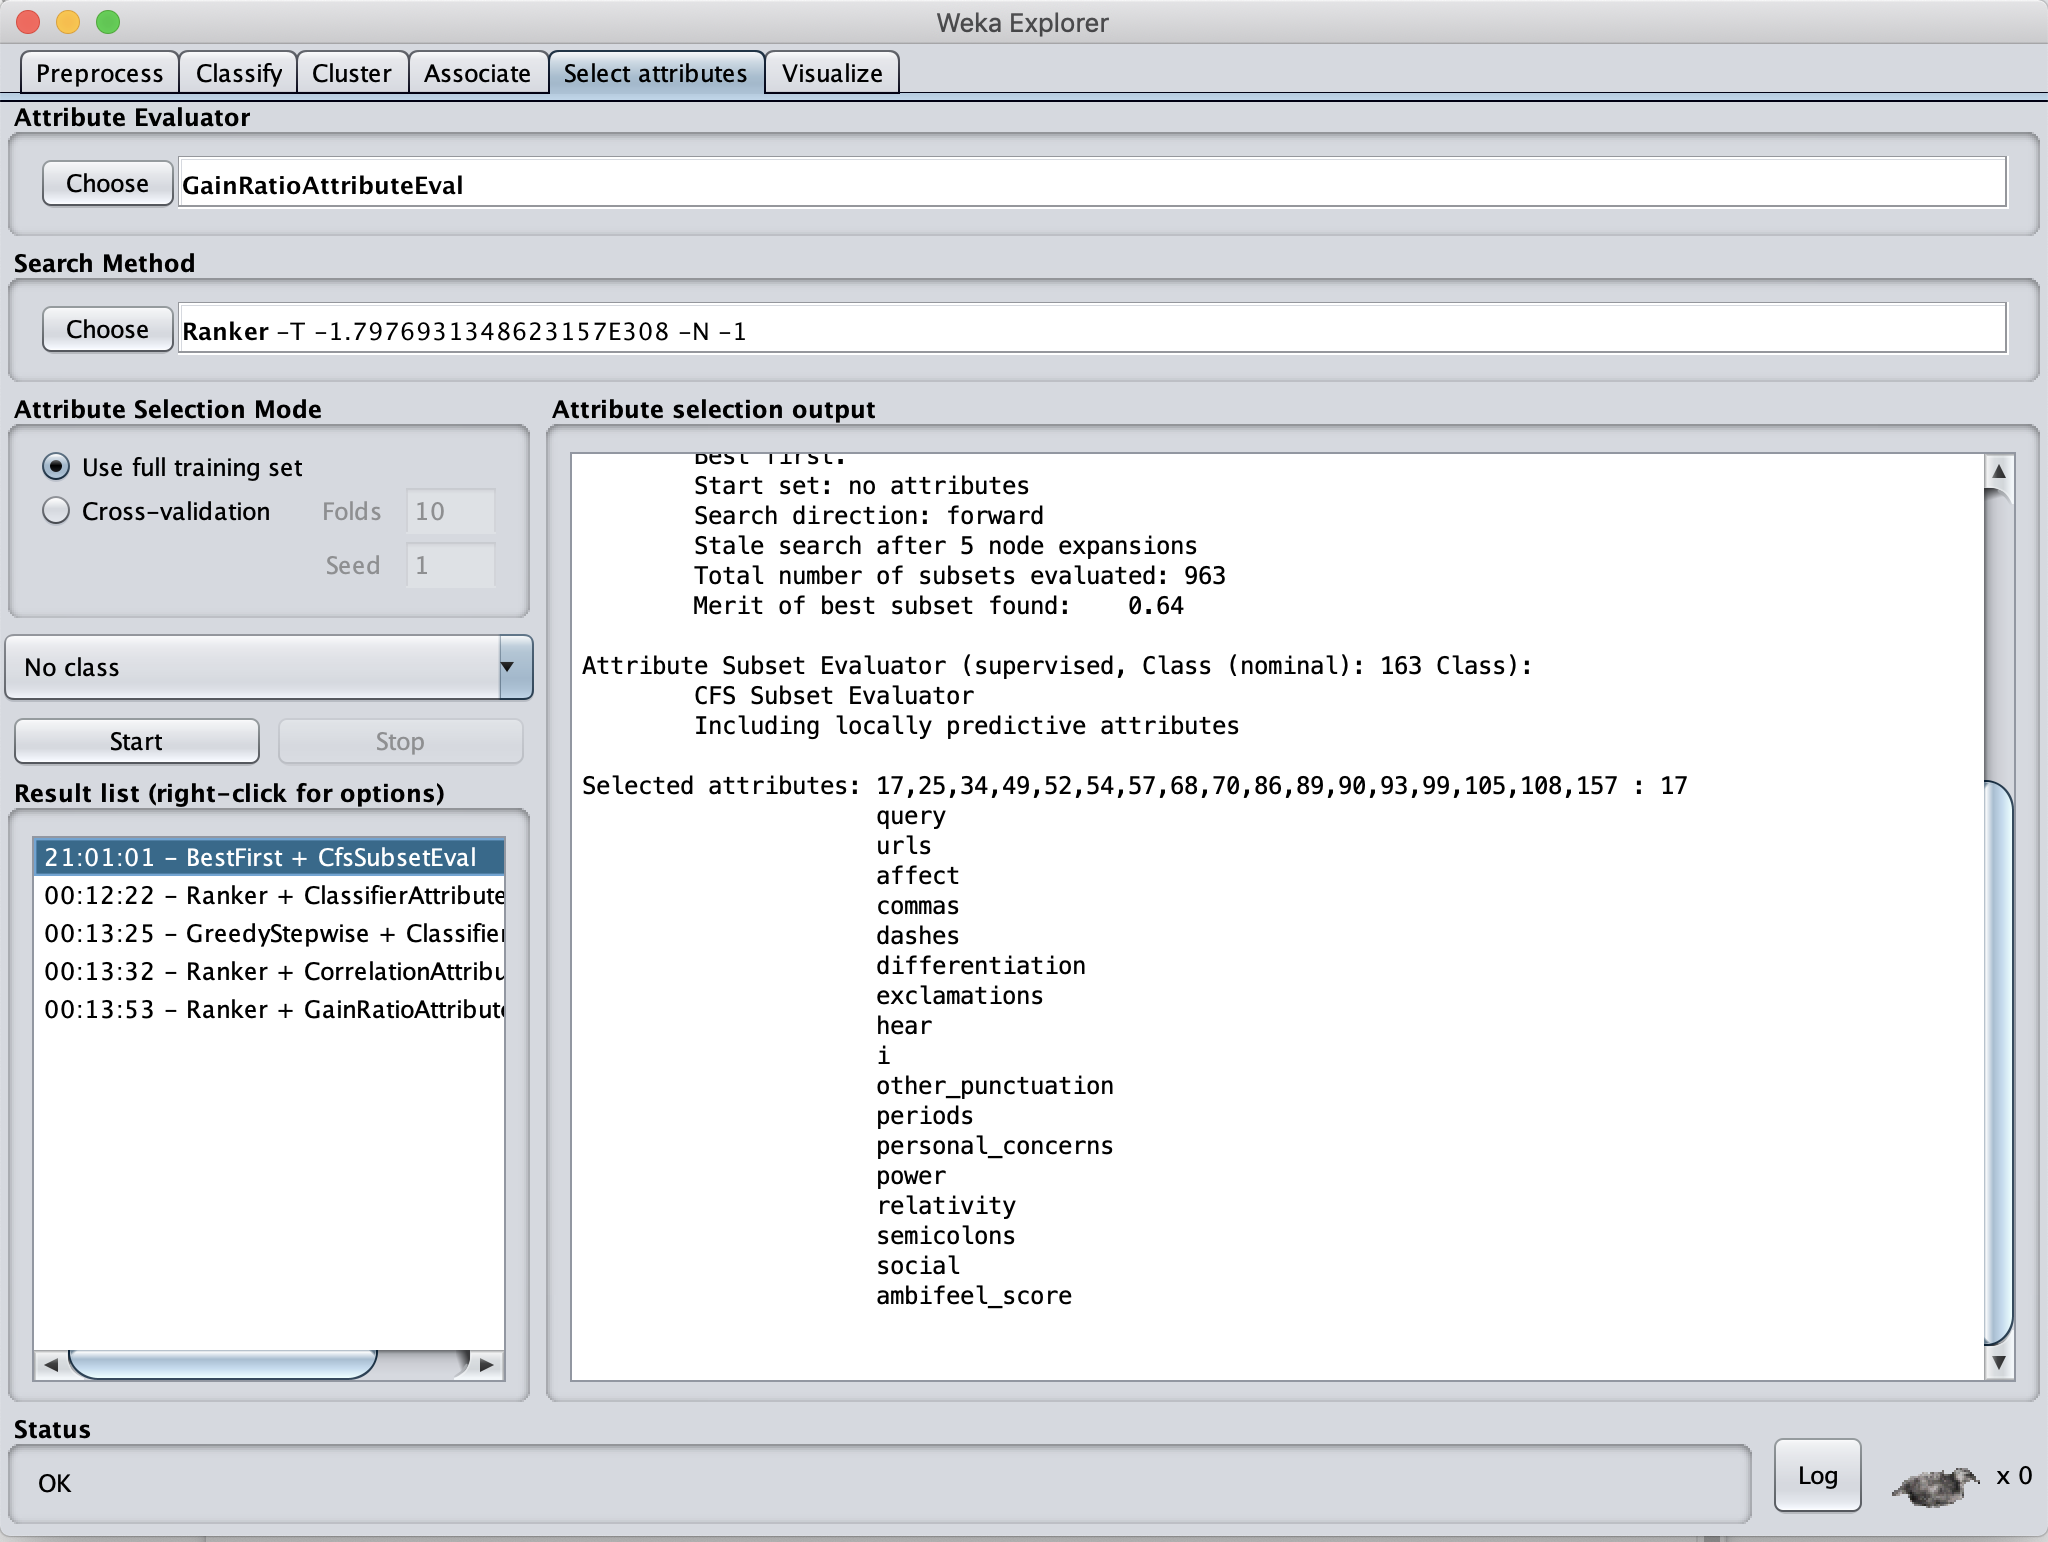
\includegraphics[width=15cm, height=12cm]{Cfs.png}
\caption{Features selected by the CfsSubsetEval Attribute Evaluator}
\end{figure}

Finally, the best score of all was obtained by using a LMT classifier with the 17 features obtained by theCfsSubsetEval Attribute Evaluator.

\begin{figure}[hbt!]
\centering
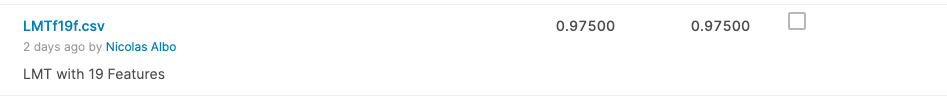
\includegraphics[width=12cm, height=1.5cm]{LMT.png}
\caption{Personal highest score obtained by using a LMT classifier with 17 features}
\end{figure}

\section{Conclusion}
Different classifiers and features were used in this work, but definitely what made the biggest impact throughout the task of building a fake news detector was the incorporation of linguistic features, specifically LIWC features. As it was explained in the Experimental Results and Discussion section, a major improvement was observed when linguistic features from the API of Receptivity were added to the list.

Different classifiers were used after the Attribute Evaluator process, but the one who had the best performance was LMT with 0.97500. The same classifier was used with Adaboost and Bagging approaches, but none of them got a better score.

%
% ---- Bibliography ----
%
% BibTeX users should specify bibliography style 'splncs04'.
% References will then be sorted and formatted in the correct style.
%
% \bibliographystyle{splncs04}
% \bibliography{mybibliography}
%
\printbibliography
\end{document}
